\section{Perturb and observe implementation}\label{MPPTImplementation}

The basic operation of the P\&O algorithm consists of perturbing the operating voltage of the PV module by means of the variation of the duty cycle of the DC-DC converter. After each perturbation the power generated by the PV module is measured (observed) and stored in order to compare it with the previous value of the power. Based on the result of the comparison, the MPP can be tracked by deciding whether the panel's voltage should be increased or decreased in the following perturbation.

There are different techniques for implementing the P\&O algorithm according to the value of the variable controlled by the MPPT and also whether the perturb value is fixed or variable \cite{implementationPandO}. The conventional P\&O algorithm uses a fixed perturb to generate a voltage or current reference signal for the outer control loop. The outer loop is used to control the switching of the DC-DC converter. Another way of implementing the conventional P\&O algorithm is using an adaptive perturb. An example of this could be setting the initial perturbation to 10\% of the $V_{oc}$, after each iteration this value is decreased by 50\% until it reaches 0.5\% of $V_{oc}$ \cite{implementationPandO}. A different technique consists of using the duty cycle of the converter as the variable controlled by the MPPT unit. Therefore, it is not necessary to implement the outer control loop. This technique can also be implemented using fixed or variable perturb step \cite{implementationPandO}. 

The P\&O algorithm that will be implemented in this project is the MPPT controlling directly the duty cycle and using a variable perturb step. It was decided to directly control the duty cycle to simplify the control system. On the other hand, an adaptive perturb is selected instead of a fixed one. The reason is that the MPPT takes longer time to reach the MPP, if a small perturb step is implemented. However, using a large perturb step the tracking would be faster but the oscillations around the MPP would be higher \cite{implementationPandO}. For this reason, it was decided to start with a perturbation step of 10\% of the $V_{oc}$ until the system reaches a certain value close to the MPP. At this point the perturbation step is iteratively reduced to one third of its previous value in order to reach accurately the MPP with lower oscillations. Figure \ref{BD_POalgorithm} shows the implementation of the system in PLECS including the MPPT which operates at a frequency of 100 Hz. 

\begin{figure}[H]
	\begin{center}
		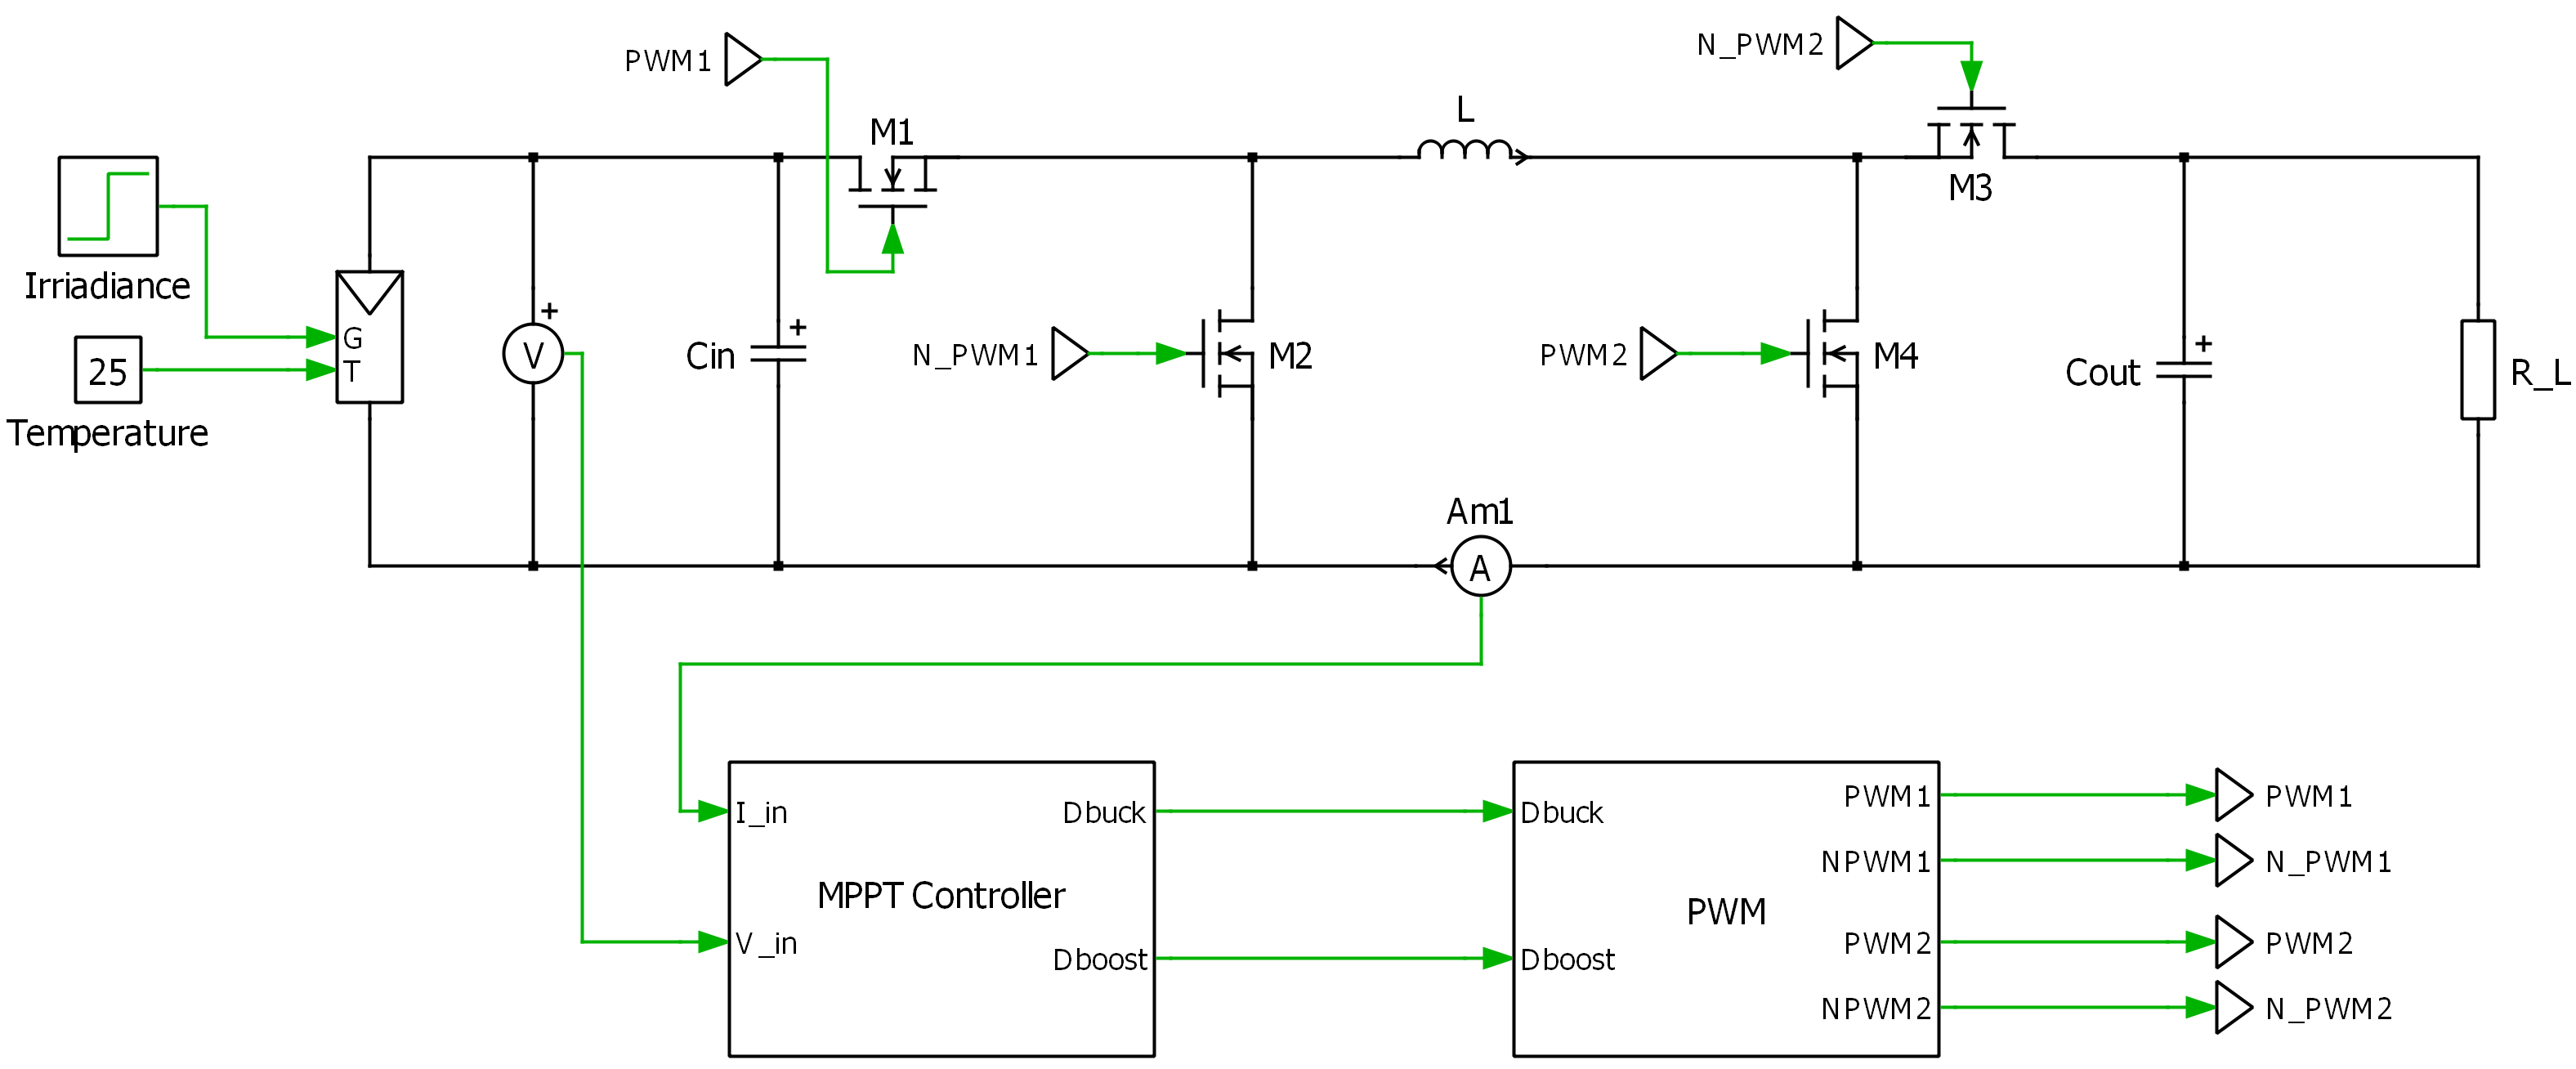
\includegraphics[width=1\textwidth]{../Pictures/BD_implementation_POalgorithm}
		\caption{Block diagram of the system including the MPPT.}
		\label{BD_POalgorithm}
	\end{center}	
\end{figure}

From the previous figure it is observed that the outputs of the MPPT block are the corresponding duty cycles for buck and boost mode. 

In order to manage these duties, a control variable called \textit{valg} has been created. It corresponds to the DC conversion ratio of the power converter ($V_{o}/V_{i}$). The conversion ratio has a different dependence on the duty when the MIC is operating in buck or in boost mode. This is shown in equations \ref{tfbuck} and \ref{tfboost}, respectively. 

The control variable \textit{valg} will be changed to increase or decrease the voltage from the PV panel. When increasing the control variable \textit{valg}, the PV voltage decreases and vice versa.
By plotting the corresponding conversion ratios and mapping them as shown in figure \ref{fig:mappingtf}, it is possible to obtain the corresponding duty cycle for the buck or the boost mode. If the control variable from the MPPT is lower than 0.5, it  means that the output voltage is lower than the input voltage and thus, the converter will work as a buck converter with duty cycle $D_{buck}=2 \cdot valg$. On the other hand, if the control variable is $valg \geq 0.5$, the output voltage is higher or equal than the input voltage and, therefore, the converter will operate in boost mode with duty cycle $D_{boost}=2\cdot valg - 1$. %These duty cycles are used to generate the corresponding PWM signals according to the converter's mode of operation at each time. 

\vspace{1cm}
\begin{minipage}{0.3\linewidth}
	\begin{equation}	\label{tfbuck}
	\frac{V_o}{V_i} = D_{buck}
	\end{equation}

\end{minipage}%
\begin{minipage}{0.5\linewidth}	
	\begin{equation}	\label{tfboost}
	\frac{V_o}{V_i}= \frac{1}{1-D_{boost}}
	\end{equation}

\end{minipage}

\begin{figure}[H]
	\begin{center}
		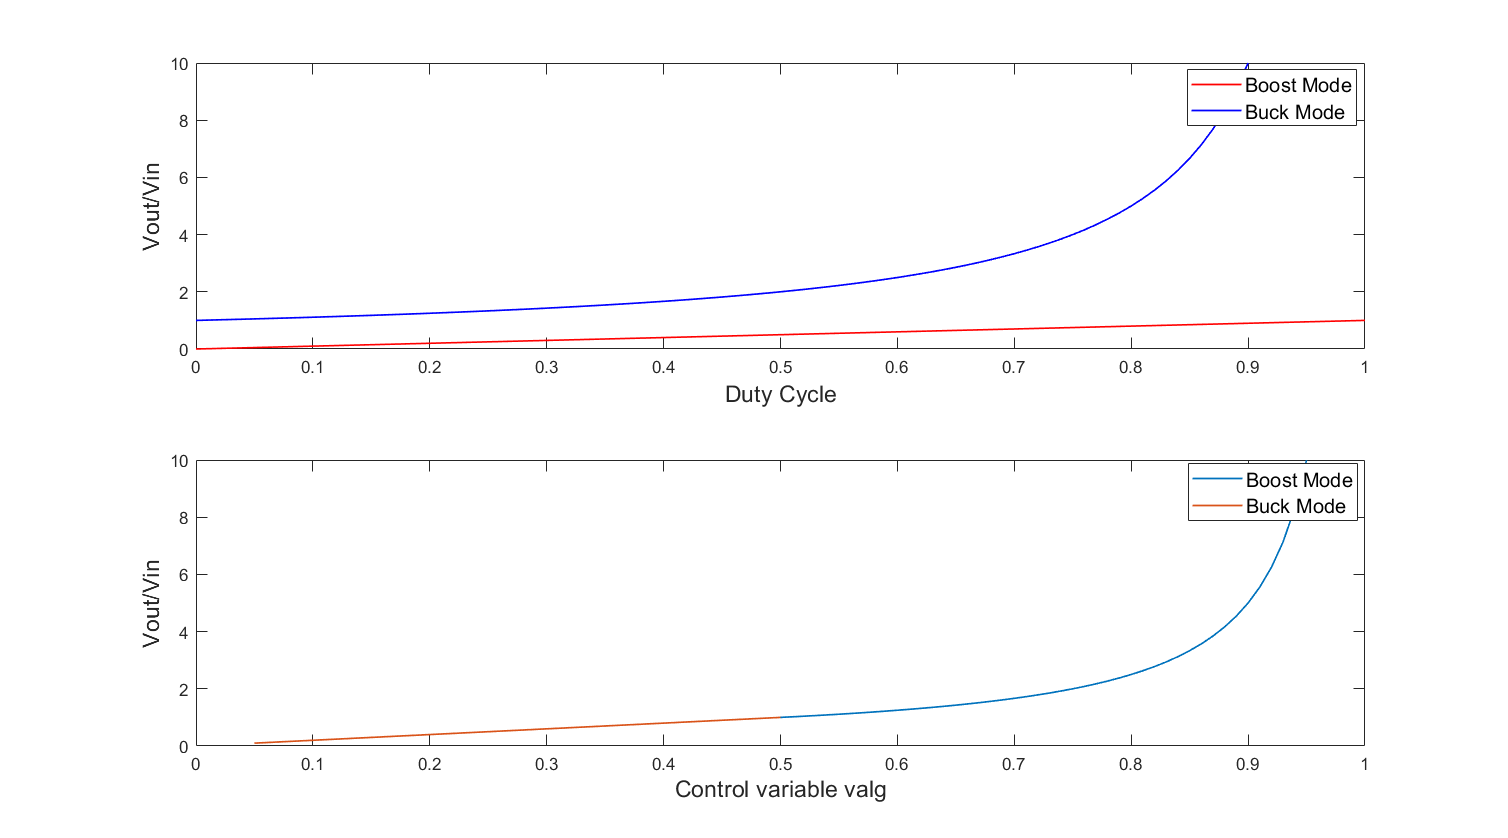
\includegraphics[width=1\textwidth]{../Pictures/decision_mode_operation}
		\caption{Top figure: Conversion ratio for buck and boost modes. Bottom figure: Mapping of the control variable valg for mode decision.}
		\label{fig:mappingtf} 
	\end{center}	
\end{figure}

The flow chart used for the implementation of the P\&O algorithm is shown in figure \ref{fcfinal}. It can be observed that the MPPT is enabled when the panel's voltage has reached the value of the open-circuit voltage. This means that the MPPT detects that the difference between the measured voltage and the previous voltage is lower than 0.1. The MPPT is forced to start at this point to be close to the value of the MPP. 
Then it starts the open-loop behavior. This is done to make the MPPT faster since the algorithm starts with $valg = 0$. The open-loop calculation decreases the voltage without evaluating the voltage and power. The condition for starting the MPPT evaluation is that $counter=15$ to ensure that the point of operation is closer to the MPP. 

It is important to notice from figure \ref{BD_POalgorithm} that the current measurement is carried out in the inductor instead of in the PV panel. This is done for possible future implementation of an outer control loop. For this reason, it is necessary to transform the measured current in order to get the corresponding measurement for the PV module's current. This current transformation is just necessary in the case of buck mode as explained in section \ref{current_sensor}. If the MPPT detects that the converter is working in buck mode, it multiplies the measured current by the corresponding duty cycle $D_{buck}=2\cdot valg$. In boost mode the average current through the inductor corresponds to the PV module's current. 

The operation of the algorithm, shown in figure \ref{fcfinal}, is an iterative process. The PV panel's voltage and power, before and after applying a voltage perturbation, are compared  in order to locate the point of operation. This way it is possible to decide if the panel's voltage has to be increased or decreased. Based on the PV characteristic curve shown in figure \ref{fig:mpp}, the following situations can occur:

\begin{enumerate}
	\item Increment of voltage and increment of power means that the point of operation is located to the left of the MPP. Therefore, the perturbance continues in the same direction (voltage is increased) with a fixed perturb step. 
	\item Increment of voltage and decrement of power means that the point of operation of the panel has gone from being located to the left of the MPP to the right of it. Therefore, the next perturbance is in the opposite direction (voltage is decreased) with a perturb step of one third of the previous step value.
	\item Decrement of voltage and increment of power means that the operation point is located to the right of the MPP. Therefore, the perturbance continues in the same direction (voltage is decreased) with a fixed perturb step. 
	\item Decrement of voltage and decrement of power means that the point of operation of the panel has changed from being located to the right of the MPP to the left of it. Therefore, the next perturbance is in the opposite direction (voltage is increased) with a perturb step os one third of the previous step value.
\end{enumerate}

After the process, once the MPP has been reached, the algorithm oscillates around this optimal point of operation. However in this case, as a variable perturb step is applied, the oscillations around the MPP will be much lower than using fixed perturb step.  

\todo{add ref to comparison, also include the comparison somewhere at the end of this chapter, before changing irradiance and temperature.}

\todo{delete valg min and valg max on initial conditions.}

\begin{figure}[H]
	\begin{center}
		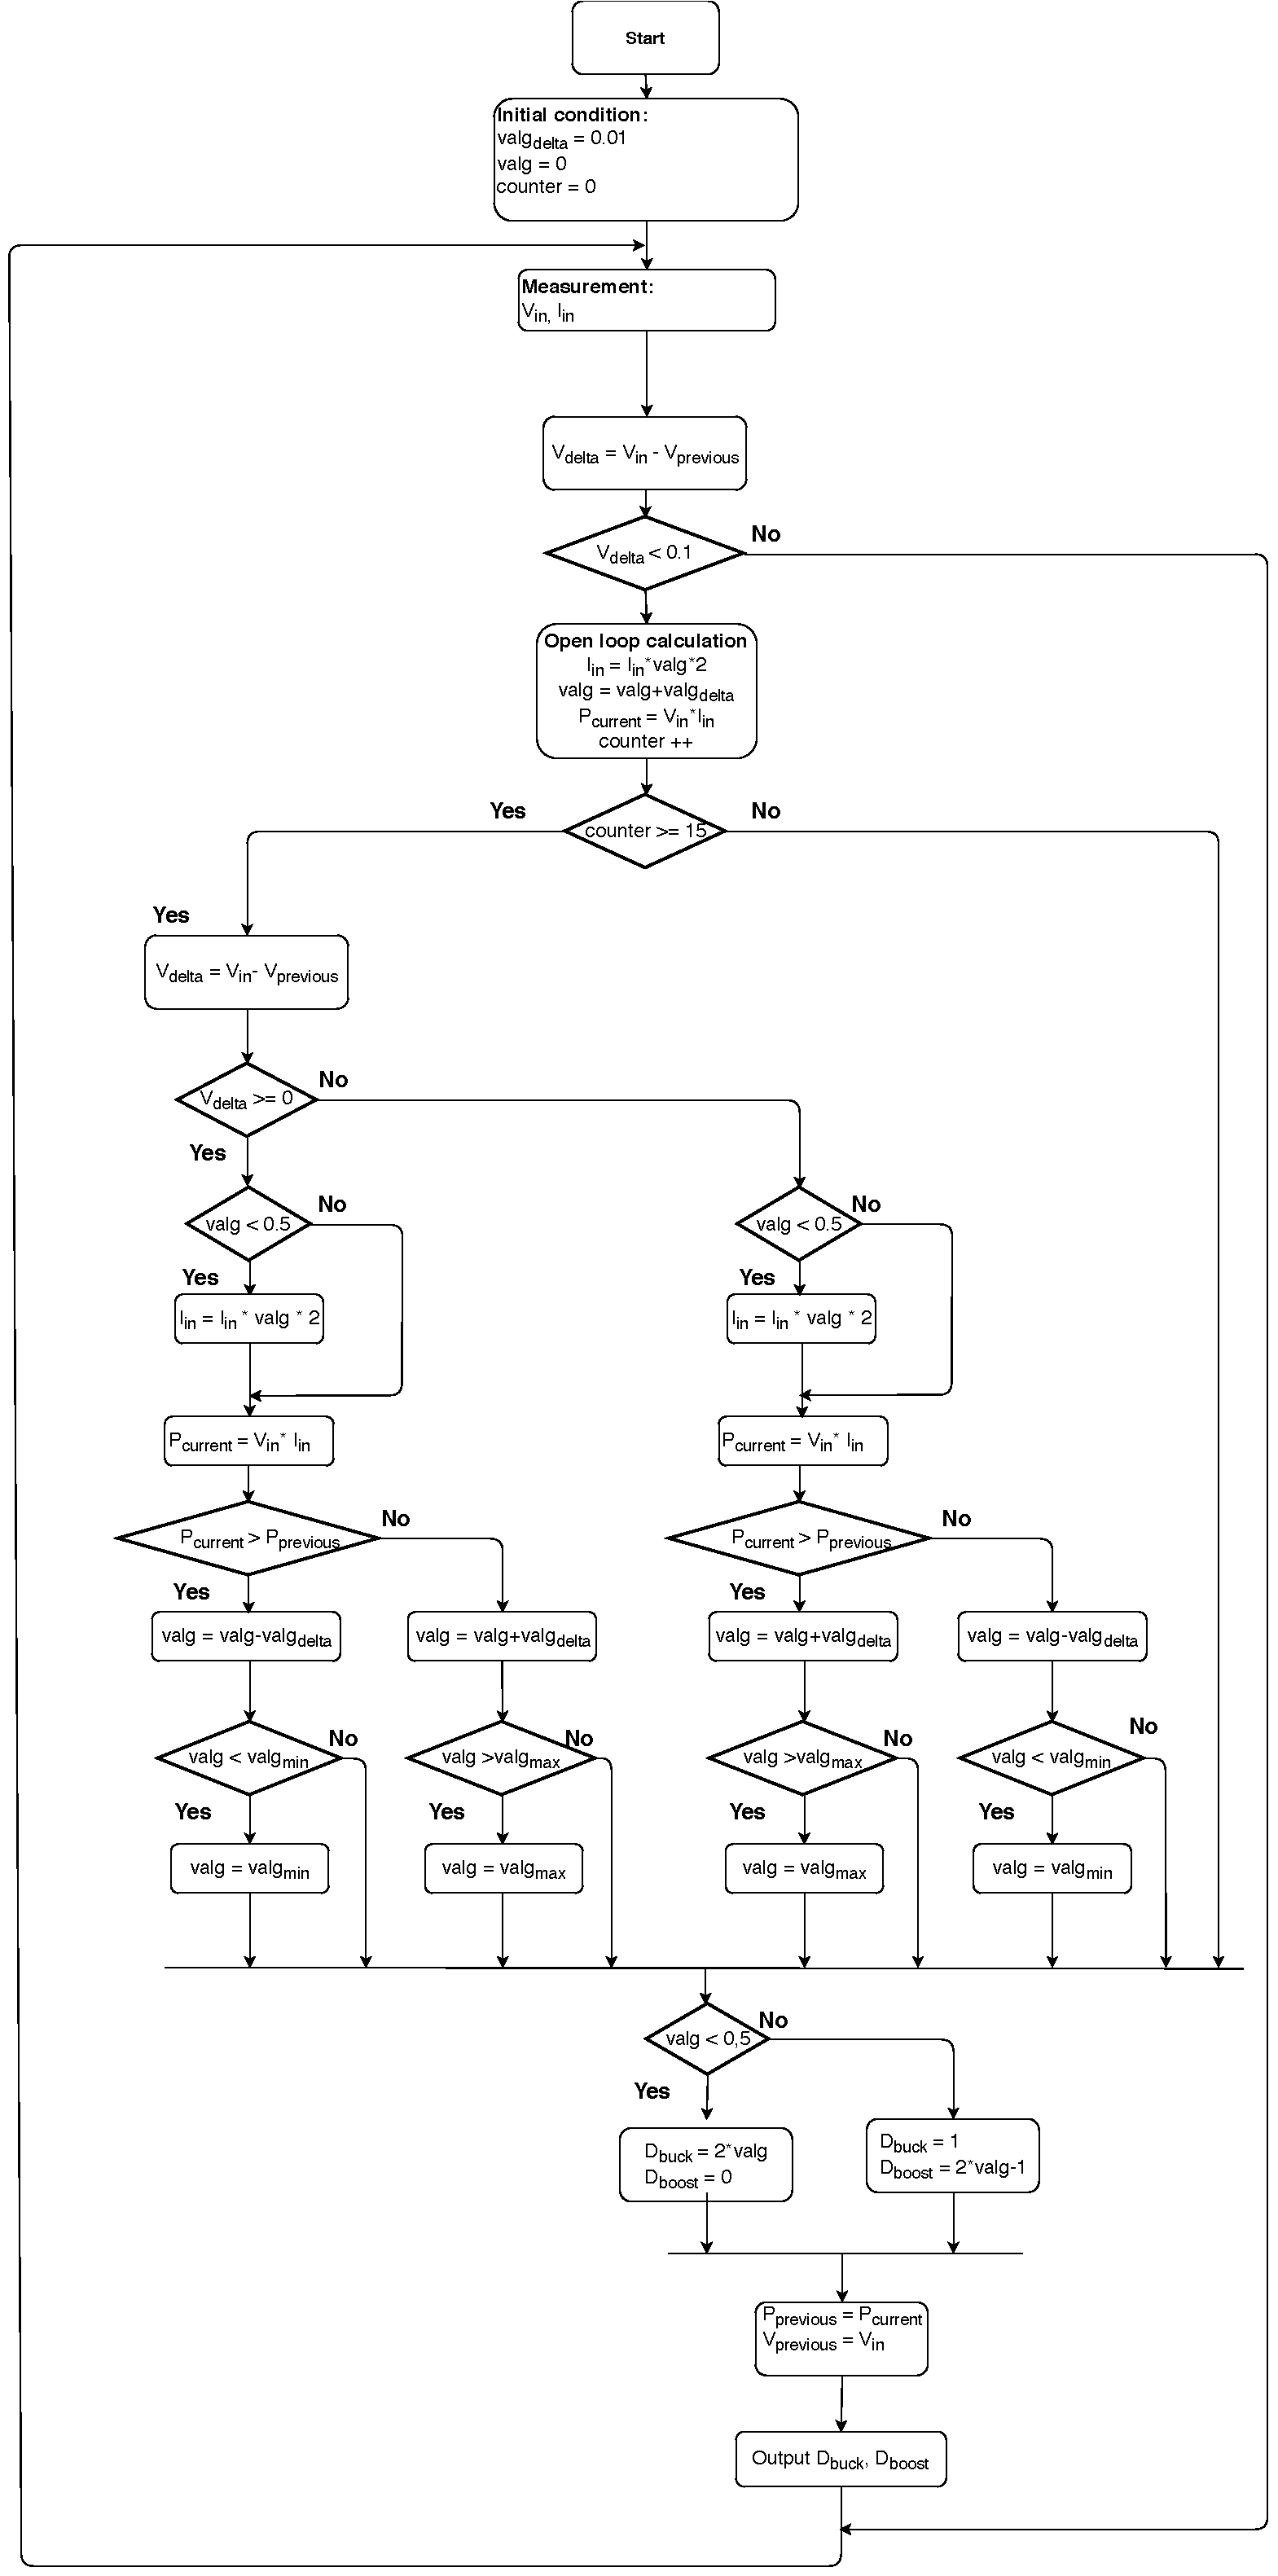
\includegraphics[width=0.87\textwidth]{../Pictures/P1/Flow_chart/2018_12_17Flow_chart_MPPT_Buck_Boost_converter.pdf}
		\caption{Flow chart for the Perturb \& Observe algorithm.}
		\label{fcfinal} 
	\end{center}	
\end{figure}

\iffalse
THINGS TO CHANGE IN THE ALGORITHM (code and flow chart):
\begin{itemize}
	\item Dmin=0.05 and Dmax=0.95 not necessary as D is not duty cycle! Check everywhere to change D for control variable. 
	\item Logic for the reset of deltaD when the system detects a change in irradiance. I think we shouldn't include this condition in the flow chart we can just show the results in graphs (in the next section) and we make the flow chart easier to read and just showing the main code. 
	\item Not necessary the start counter because with the counter for the open loop calculation the MPPT is enabled after the Voc has been reached. 
\end{itemize}
\fi


